\documentclass[11pt]{article}
\usepackage[margin=0.75in]{geometry}
\usepackage{amsmath}
\usepackage{enumitem}
\usepackage{color,soul}
\usepackage{multicol}
\usepackage{tikz}

\newcommand{\ds}{\displaystyle}

\begin{document}
\newcounter{enumCount}
\pagestyle{empty}
\subsection*{Math 141 - Homework 11 \hfill Name: \underline{\hspace*{2in}}}


\textit{Solve each of the following optimization problems.  Be sure to include confirmation that your solution is really the maximum or the minimum (use the first or second derivative test).}

\begin{enumerate}
\item Two poles are connected by a wire that is also
connected to the ground. The first pole is 20 ft tall and
the second pole is 10 ft tall. There is a distance of 30 ft
between the two poles. Where should the wire be anchored
to the ground to minimize the amount of wire needed?
\begin{flushright}
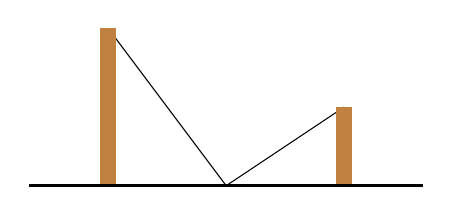
\begin{tikzpicture}
\draw (3,1) -- (1.5,0) -- (0,2);
\fill[brown] (-0.1,0) rectangle (0.1,2);
\fill[brown] (2.9,0) rectangle (3.1,1);
\draw[very thick] (-1,0) -- (4,0);
\end{tikzpicture}
\end{flushright}
\vfill

\item The sum of two positive numbers is 10.  Find the values of the numbers that maximize their product.  
\vfill
\vfill

\item What point on the line $3x + 4y = 50$ is closest to the origin? 
\vfill
\vfill

\item A Norman window is a rectangle with a half-circle on top. If the perimeter of the window is 20 feet, find the dimensions $r$ and $h$ for the Norman window that has the largest possible area. 
\begin{flushright}
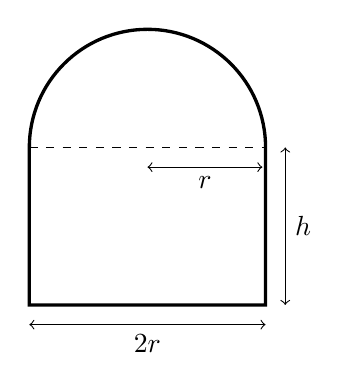
\begin{tikzpicture}
\draw[very thick] (0,0) -- (3,0) -- (3,2) arc (0:180:1.5) -- cycle;
\draw[dashed] (0,2) -- (3,2);
\draw[<->] (0,-0.25) -- (1.5,-0.25) node[below] {$2r$} -- (3,-0.25);
\draw[<->] (1.5,1.75) -- (2.23,1.75) node[below] {$r$} -- (2.96,1.75);
\draw[<->] (3.25,0) -- (3.25,1) node[right] {$h$} -- (3.25,2);
\end{tikzpicture}
\end{flushright}

\newpage


\end{enumerate}

\end{document}
